% Options for packages loaded elsewhere
% Options for packages loaded elsewhere
\PassOptionsToPackage{unicode}{hyperref}
\PassOptionsToPackage{hyphens}{url}
\PassOptionsToPackage{dvipsnames,svgnames,x11names}{xcolor}
%
\documentclass[
  letterpaper,
  DIV=11,
  numbers=noendperiod]{scrartcl}
\usepackage{xcolor}
\usepackage{amsmath,amssymb}
\setcounter{secnumdepth}{-\maxdimen} % remove section numbering
\usepackage{iftex}
\ifPDFTeX
  \usepackage[T1]{fontenc}
  \usepackage[utf8]{inputenc}
  \usepackage{textcomp} % provide euro and other symbols
\else % if luatex or xetex
  \usepackage{unicode-math} % this also loads fontspec
  \defaultfontfeatures{Scale=MatchLowercase}
  \defaultfontfeatures[\rmfamily]{Ligatures=TeX,Scale=1}
\fi
\usepackage{lmodern}
\ifPDFTeX\else
  % xetex/luatex font selection
\fi
% Use upquote if available, for straight quotes in verbatim environments
\IfFileExists{upquote.sty}{\usepackage{upquote}}{}
\IfFileExists{microtype.sty}{% use microtype if available
  \usepackage[]{microtype}
  \UseMicrotypeSet[protrusion]{basicmath} % disable protrusion for tt fonts
}{}
\makeatletter
\@ifundefined{KOMAClassName}{% if non-KOMA class
  \IfFileExists{parskip.sty}{%
    \usepackage{parskip}
  }{% else
    \setlength{\parindent}{0pt}
    \setlength{\parskip}{6pt plus 2pt minus 1pt}}
}{% if KOMA class
  \KOMAoptions{parskip=half}}
\makeatother
% Make \paragraph and \subparagraph free-standing
\makeatletter
\ifx\paragraph\undefined\else
  \let\oldparagraph\paragraph
  \renewcommand{\paragraph}{
    \@ifstar
      \xxxParagraphStar
      \xxxParagraphNoStar
  }
  \newcommand{\xxxParagraphStar}[1]{\oldparagraph*{#1}\mbox{}}
  \newcommand{\xxxParagraphNoStar}[1]{\oldparagraph{#1}\mbox{}}
\fi
\ifx\subparagraph\undefined\else
  \let\oldsubparagraph\subparagraph
  \renewcommand{\subparagraph}{
    \@ifstar
      \xxxSubParagraphStar
      \xxxSubParagraphNoStar
  }
  \newcommand{\xxxSubParagraphStar}[1]{\oldsubparagraph*{#1}\mbox{}}
  \newcommand{\xxxSubParagraphNoStar}[1]{\oldsubparagraph{#1}\mbox{}}
\fi
\makeatother

\usepackage{color}
\usepackage{fancyvrb}
\newcommand{\VerbBar}{|}
\newcommand{\VERB}{\Verb[commandchars=\\\{\}]}
\DefineVerbatimEnvironment{Highlighting}{Verbatim}{commandchars=\\\{\}}
% Add ',fontsize=\small' for more characters per line
\usepackage{framed}
\definecolor{shadecolor}{RGB}{241,243,245}
\newenvironment{Shaded}{\begin{snugshade}}{\end{snugshade}}
\newcommand{\AlertTok}[1]{\textcolor[rgb]{0.68,0.00,0.00}{#1}}
\newcommand{\AnnotationTok}[1]{\textcolor[rgb]{0.37,0.37,0.37}{#1}}
\newcommand{\AttributeTok}[1]{\textcolor[rgb]{0.40,0.45,0.13}{#1}}
\newcommand{\BaseNTok}[1]{\textcolor[rgb]{0.68,0.00,0.00}{#1}}
\newcommand{\BuiltInTok}[1]{\textcolor[rgb]{0.00,0.23,0.31}{#1}}
\newcommand{\CharTok}[1]{\textcolor[rgb]{0.13,0.47,0.30}{#1}}
\newcommand{\CommentTok}[1]{\textcolor[rgb]{0.37,0.37,0.37}{#1}}
\newcommand{\CommentVarTok}[1]{\textcolor[rgb]{0.37,0.37,0.37}{\textit{#1}}}
\newcommand{\ConstantTok}[1]{\textcolor[rgb]{0.56,0.35,0.01}{#1}}
\newcommand{\ControlFlowTok}[1]{\textcolor[rgb]{0.00,0.23,0.31}{\textbf{#1}}}
\newcommand{\DataTypeTok}[1]{\textcolor[rgb]{0.68,0.00,0.00}{#1}}
\newcommand{\DecValTok}[1]{\textcolor[rgb]{0.68,0.00,0.00}{#1}}
\newcommand{\DocumentationTok}[1]{\textcolor[rgb]{0.37,0.37,0.37}{\textit{#1}}}
\newcommand{\ErrorTok}[1]{\textcolor[rgb]{0.68,0.00,0.00}{#1}}
\newcommand{\ExtensionTok}[1]{\textcolor[rgb]{0.00,0.23,0.31}{#1}}
\newcommand{\FloatTok}[1]{\textcolor[rgb]{0.68,0.00,0.00}{#1}}
\newcommand{\FunctionTok}[1]{\textcolor[rgb]{0.28,0.35,0.67}{#1}}
\newcommand{\ImportTok}[1]{\textcolor[rgb]{0.00,0.46,0.62}{#1}}
\newcommand{\InformationTok}[1]{\textcolor[rgb]{0.37,0.37,0.37}{#1}}
\newcommand{\KeywordTok}[1]{\textcolor[rgb]{0.00,0.23,0.31}{\textbf{#1}}}
\newcommand{\NormalTok}[1]{\textcolor[rgb]{0.00,0.23,0.31}{#1}}
\newcommand{\OperatorTok}[1]{\textcolor[rgb]{0.37,0.37,0.37}{#1}}
\newcommand{\OtherTok}[1]{\textcolor[rgb]{0.00,0.23,0.31}{#1}}
\newcommand{\PreprocessorTok}[1]{\textcolor[rgb]{0.68,0.00,0.00}{#1}}
\newcommand{\RegionMarkerTok}[1]{\textcolor[rgb]{0.00,0.23,0.31}{#1}}
\newcommand{\SpecialCharTok}[1]{\textcolor[rgb]{0.37,0.37,0.37}{#1}}
\newcommand{\SpecialStringTok}[1]{\textcolor[rgb]{0.13,0.47,0.30}{#1}}
\newcommand{\StringTok}[1]{\textcolor[rgb]{0.13,0.47,0.30}{#1}}
\newcommand{\VariableTok}[1]{\textcolor[rgb]{0.07,0.07,0.07}{#1}}
\newcommand{\VerbatimStringTok}[1]{\textcolor[rgb]{0.13,0.47,0.30}{#1}}
\newcommand{\WarningTok}[1]{\textcolor[rgb]{0.37,0.37,0.37}{\textit{#1}}}

\usepackage{longtable,booktabs,array}
\newcounter{none} % for unnumbered tables
\usepackage{calc} % for calculating minipage widths
% Correct order of tables after \paragraph or \subparagraph
\usepackage{etoolbox}
\makeatletter
\patchcmd\longtable{\par}{\if@noskipsec\mbox{}\fi\par}{}{}
\makeatother
% Allow footnotes in longtable head/foot
\IfFileExists{footnotehyper.sty}{\usepackage{footnotehyper}}{\usepackage{footnote}}
\makesavenoteenv{longtable}
\usepackage{graphicx}
\makeatletter
\newsavebox\pandoc@box
\newcommand*\pandocbounded[1]{% scales image to fit in text height/width
  \sbox\pandoc@box{#1}%
  \Gscale@div\@tempa{\textheight}{\dimexpr\ht\pandoc@box+\dp\pandoc@box\relax}%
  \Gscale@div\@tempb{\linewidth}{\wd\pandoc@box}%
  \ifdim\@tempb\p@<\@tempa\p@\let\@tempa\@tempb\fi% select the smaller of both
  \ifdim\@tempa\p@<\p@\scalebox{\@tempa}{\usebox\pandoc@box}%
  \else\usebox{\pandoc@box}%
  \fi%
}
% Set default figure placement to htbp
\def\fps@figure{htbp}
\makeatother





\setlength{\emergencystretch}{3em} % prevent overfull lines

\providecommand{\tightlist}{%
  \setlength{\itemsep}{0pt}\setlength{\parskip}{0pt}}



 


\KOMAoption{captions}{tableheading}
\makeatletter
\@ifpackageloaded{caption}{}{\usepackage{caption}}
\AtBeginDocument{%
\ifdefined\contentsname
  \renewcommand*\contentsname{Table of contents}
\else
  \newcommand\contentsname{Table of contents}
\fi
\ifdefined\listfigurename
  \renewcommand*\listfigurename{List of Figures}
\else
  \newcommand\listfigurename{List of Figures}
\fi
\ifdefined\listtablename
  \renewcommand*\listtablename{List of Tables}
\else
  \newcommand\listtablename{List of Tables}
\fi
\ifdefined\figurename
  \renewcommand*\figurename{Figure}
\else
  \newcommand\figurename{Figure}
\fi
\ifdefined\tablename
  \renewcommand*\tablename{Table}
\else
  \newcommand\tablename{Table}
\fi
}
\@ifpackageloaded{float}{}{\usepackage{float}}
\floatstyle{ruled}
\@ifundefined{c@chapter}{\newfloat{codelisting}{h}{lop}}{\newfloat{codelisting}{h}{lop}[chapter]}
\floatname{codelisting}{Listing}
\newcommand*\listoflistings{\listof{codelisting}{List of Listings}}
\makeatother
\makeatletter
\makeatother
\makeatletter
\@ifpackageloaded{caption}{}{\usepackage{caption}}
\@ifpackageloaded{subcaption}{}{\usepackage{subcaption}}
\makeatother
\usepackage{bookmark}
\IfFileExists{xurl.sty}{\usepackage{xurl}}{} % add URL line breaks if available
\urlstyle{same}
% fallback for those not using the hyperref driver hyperxmp:
\makeatletter
\@ifundefined{xmpquote}{\newcommand{\xmpquote}[1]{#1}}{}
\makeatother
\hypersetup{
  pdftitle={Lecture 14},
  pdfauthor={Emad Masroor},
  colorlinks=true,
  linkcolor={blue},
  filecolor={Maroon},
  citecolor={Blue},
  urlcolor={Blue},
  pdfcreator={LaTeX via pandoc}}


\title{Lecture 14}
\usepackage{etoolbox}
\makeatletter
\providecommand{\subtitle}[1]{% add subtitle to \maketitle
  \apptocmd{\@title}{\par {\large #1 \par}}{}{}
}
\makeatother
\subtitle{E21 Computer Engineering Fundamentals}
\author{Emad Masroor}
\date{October 22, 2026}
\begin{document}
\maketitle


\subsubsection{Bisection Method}\label{bisection-method}

\pandocbounded{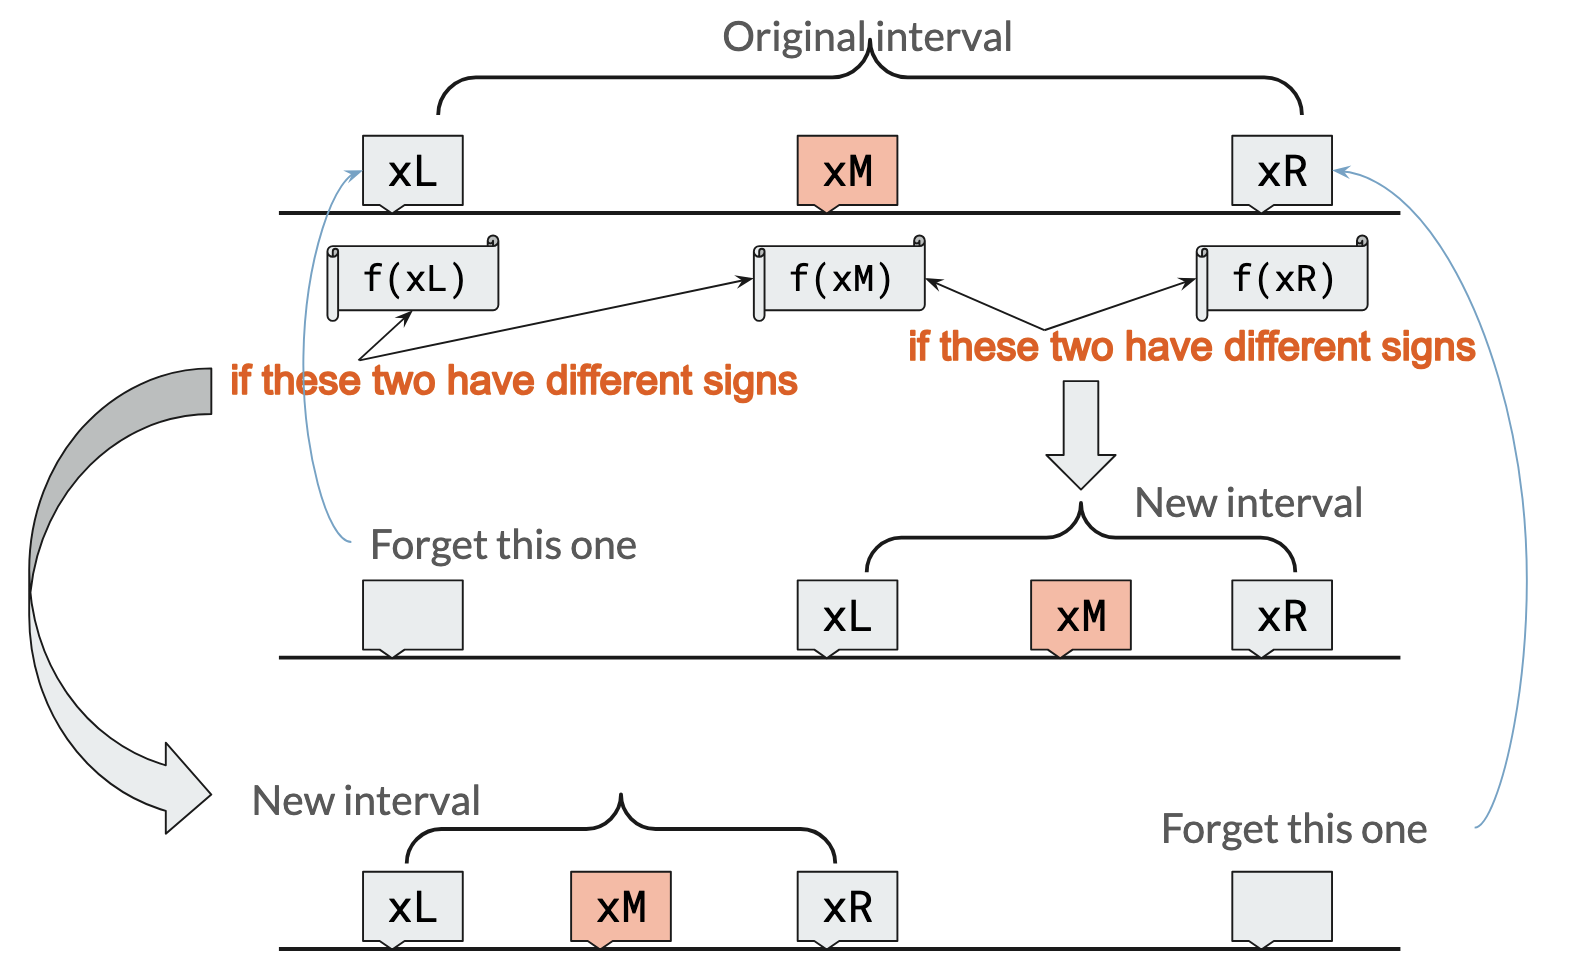
\includegraphics[keepaspectratio]{bisection.png}}

\subsubsection{Convergence rates}\label{convergence-rates}

At each subsequent bisection step, the bisection window is halved.

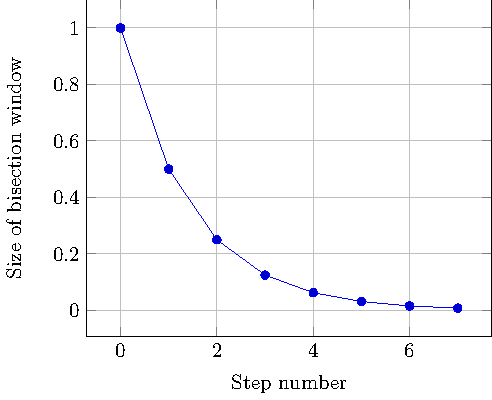
\includegraphics[width=6in,height=\textheight,keepaspectratio]{index_files/mediabag/tikz.6880ac03.pdf}

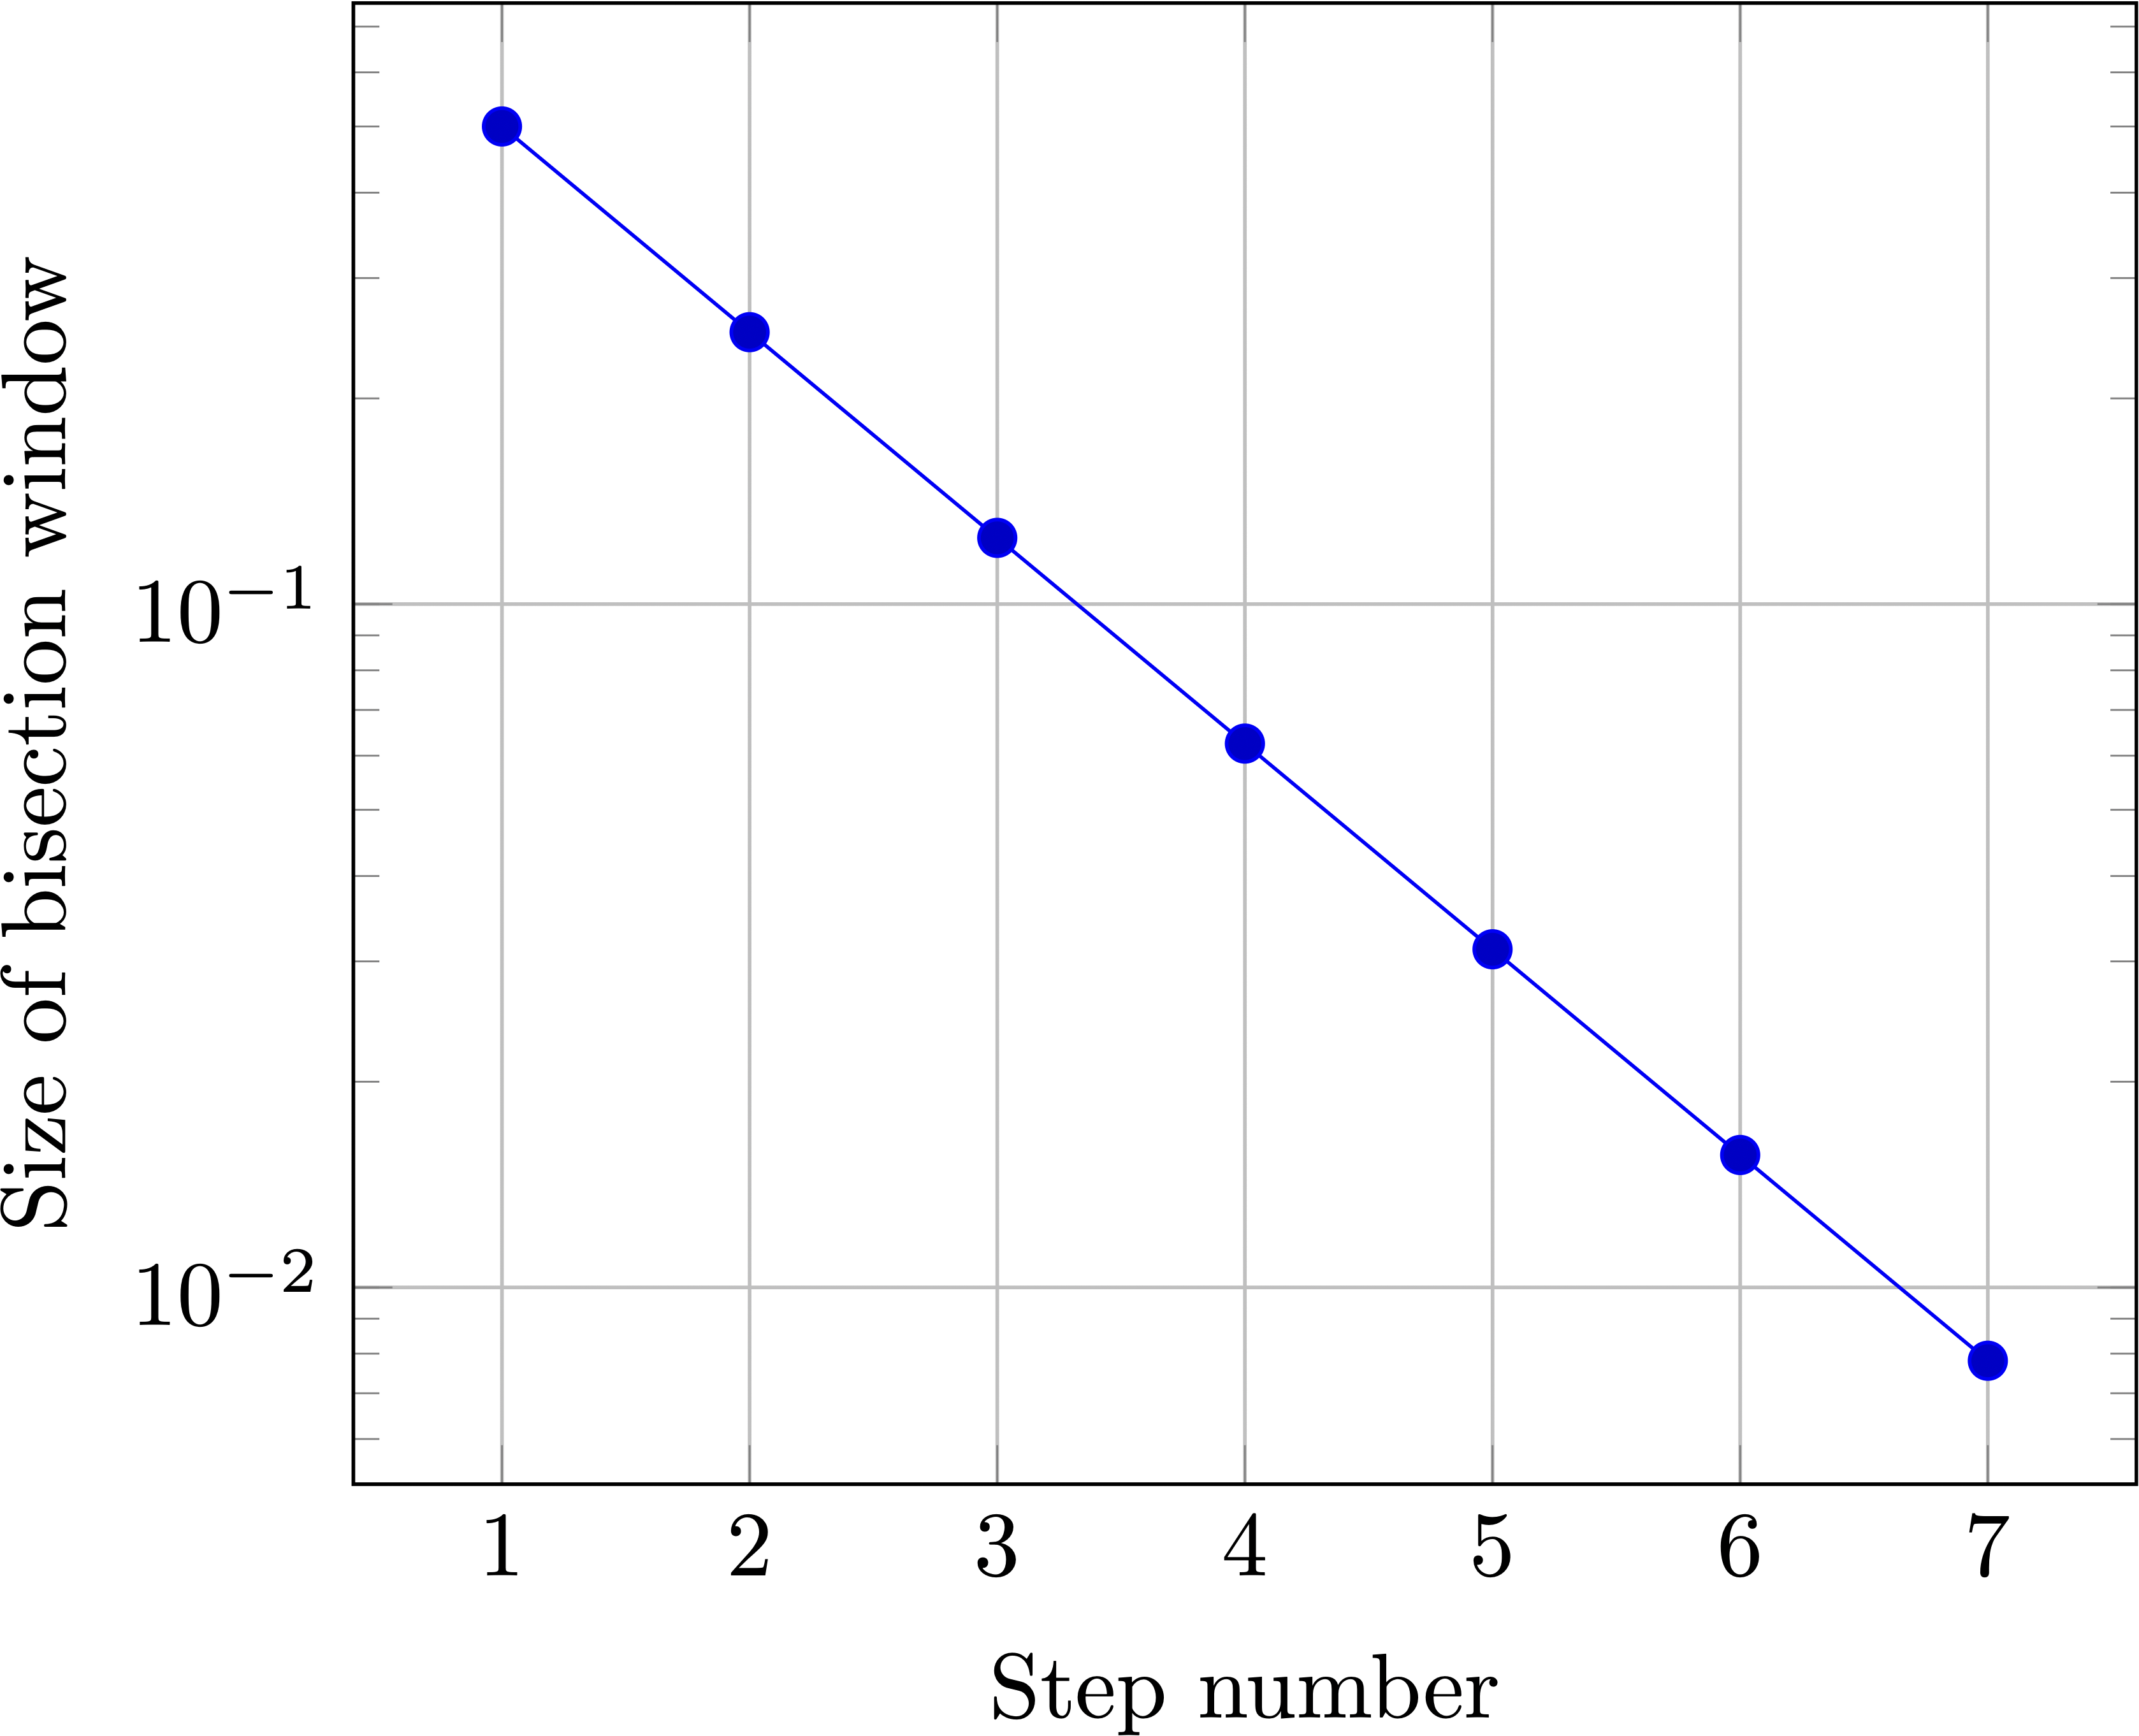
\includegraphics[width=6in,height=\textheight,keepaspectratio]{logscale.png}

\subsubsection{General approach to
root-finding}\label{general-approach-to-root-finding}

In all root-finding approaches, we:

\begin{itemize}
\tightlist
\item
  start with a guess of where the root might be,
\item
  work \textbf{iteratively}, repeatedly applying the same formula many
  times

  \begin{itemize}
  \tightlist
  \item
    the number of iterations it takes to arrive at a solution is an
    important measure of how good an approach is.
  \item
    in practice, this is either a \texttt{while} or \texttt{for} loop.
  \end{itemize}
\item
  hopefully \textbf{converge} to \emph{one} root.
\end{itemize}

\subsubsection{The Secant Method}\label{the-secant-method}

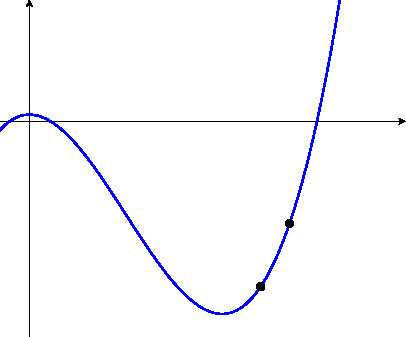
\includegraphics[width=6in,height=\textheight,keepaspectratio]{index_files/mediabag/tikz.281e83bc.pdf}

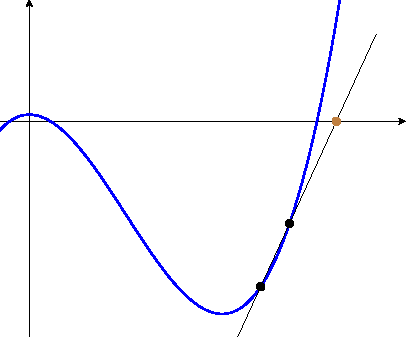
\includegraphics[width=6in,height=\textheight,keepaspectratio]{index_files/mediabag/tikz.8e8bc0e1.pdf}

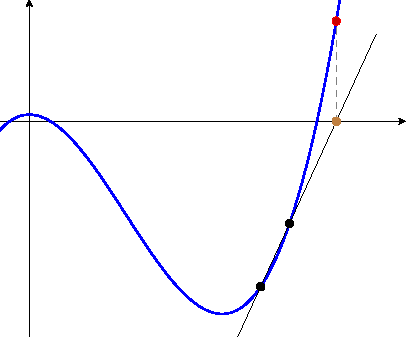
\includegraphics[width=6in,height=\textheight,keepaspectratio]{index_files/mediabag/tikz.869768f8.pdf}

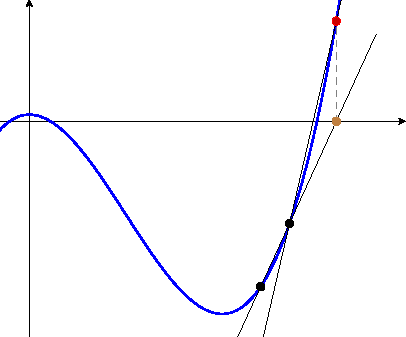
\includegraphics[width=6in,height=\textheight,keepaspectratio]{index_files/mediabag/tikz.d4a0c5b8.pdf}

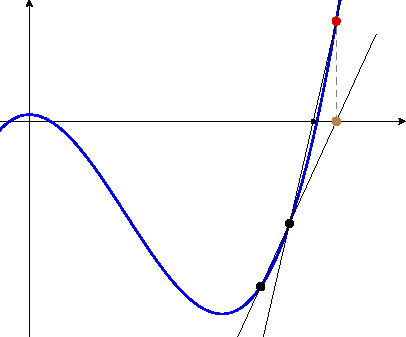
\includegraphics[width=6in,height=\textheight,keepaspectratio]{index_files/mediabag/tikz.36c811b8.pdf}

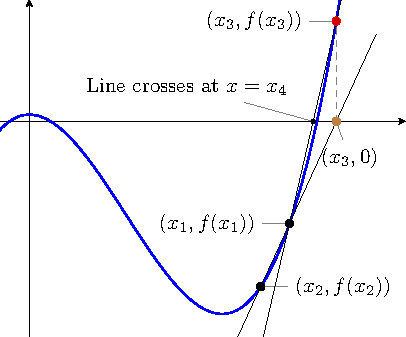
\includegraphics[width=6in,height=\textheight,keepaspectratio]{index_files/mediabag/tikz.e00a677e.pdf}

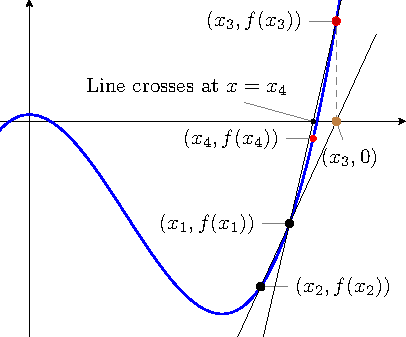
\includegraphics[width=6in,height=\textheight,keepaspectratio]{index_files/mediabag/tikz.5439d9cd.pdf}

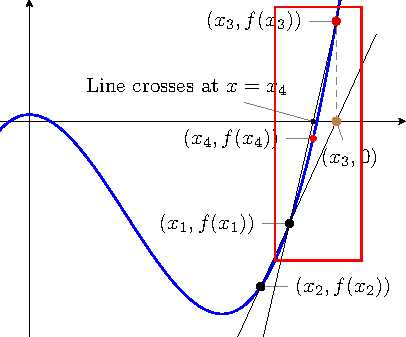
\includegraphics[width=6in,height=\textheight,keepaspectratio]{index_files/mediabag/tikz.0ba2c7ab.pdf}

\subsubsection{Secant Method --- Zoomed
in}\label{secant-method-zoomed-in}

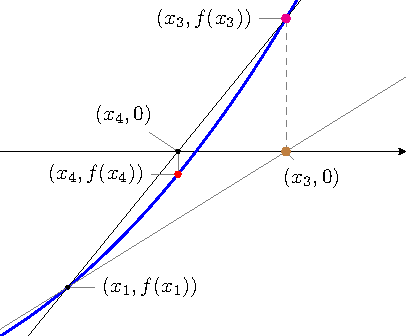
\includegraphics[width=6in,height=\textheight,keepaspectratio]{index_files/mediabag/tikz.b47dac3d.pdf}

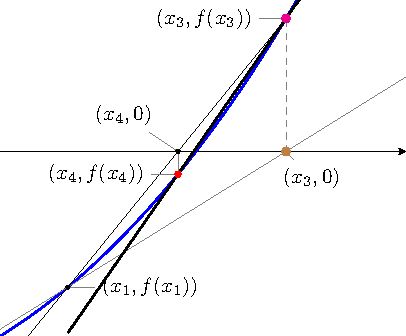
\includegraphics[width=6in,height=\textheight,keepaspectratio]{index_files/mediabag/tikz.ddda4e10.pdf}

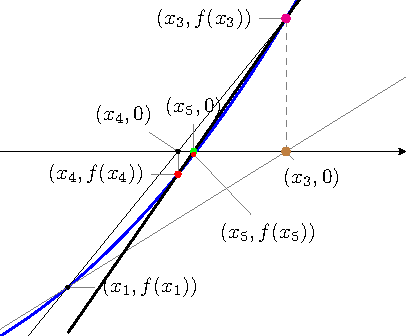
\includegraphics[width=6in,height=\textheight,keepaspectratio]{index_files/mediabag/tikz.b4681339.pdf}

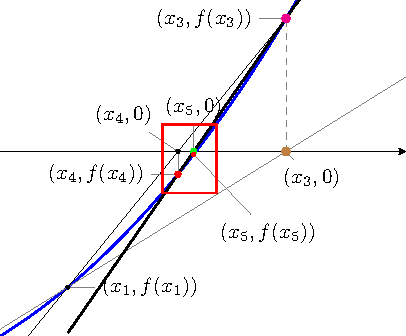
\includegraphics[width=6in,height=\textheight,keepaspectratio]{index_files/mediabag/tikz.97f0d5a7.pdf}

\subsubsection{Secant Method --- Zoomed in
again}\label{secant-method-zoomed-in-again}

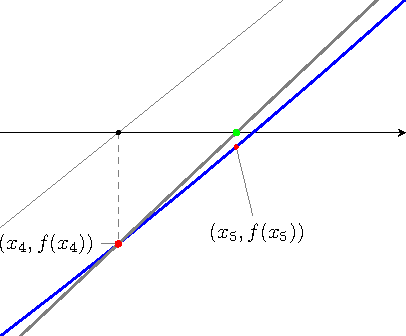
\includegraphics[width=6in,height=\textheight,keepaspectratio]{index_files/mediabag/tikz.63fa71ac.pdf}

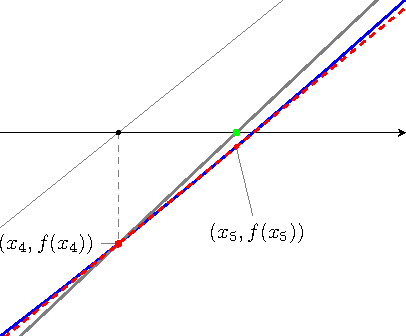
\includegraphics[width=6in,height=\textheight,keepaspectratio]{index_files/mediabag/tikz.f52b1c74.pdf}

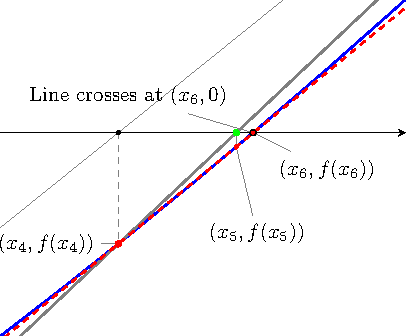
\includegraphics[width=6in,height=\textheight,keepaspectratio]{index_files/mediabag/tikz.5ec8aa3e.pdf}

\subsubsection{Summary of Secant Method}\label{summary-of-secant-method}

{Start with two estimates of the root.}

{Evaluate the function at both \(x_1\) and \(x_2\)}

{Draw a straight line between the two points. This is an estimate of the
function's behavior.}

{Locate the point \((x_3,0)\) where this line crosses the x-axis. Call
this \(x_3\).}

{Let \((x_3,f_3)\) be a new point. Forget about \((x_1,f_1)\).}

{Repeat the process above, using the points \((x_2,f_2)\) and
\((x_3,f_3)\)}

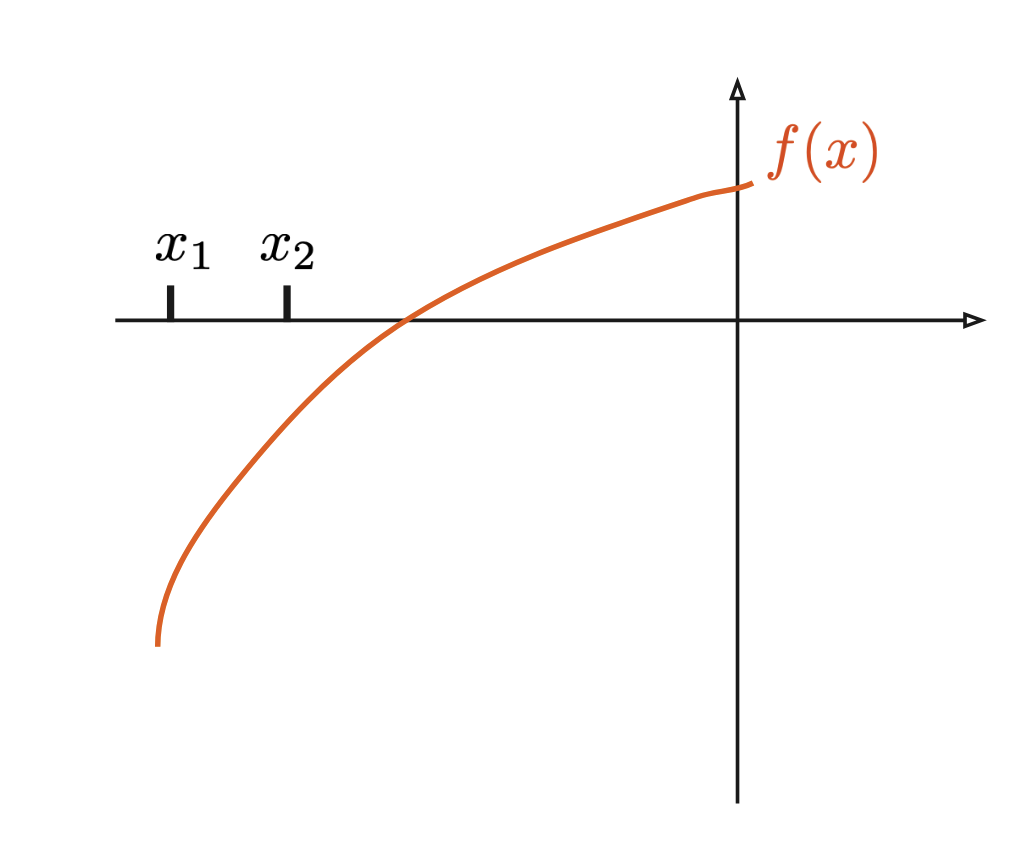
\includegraphics[width=3.64583in,height=3.125in]{sec1.png}
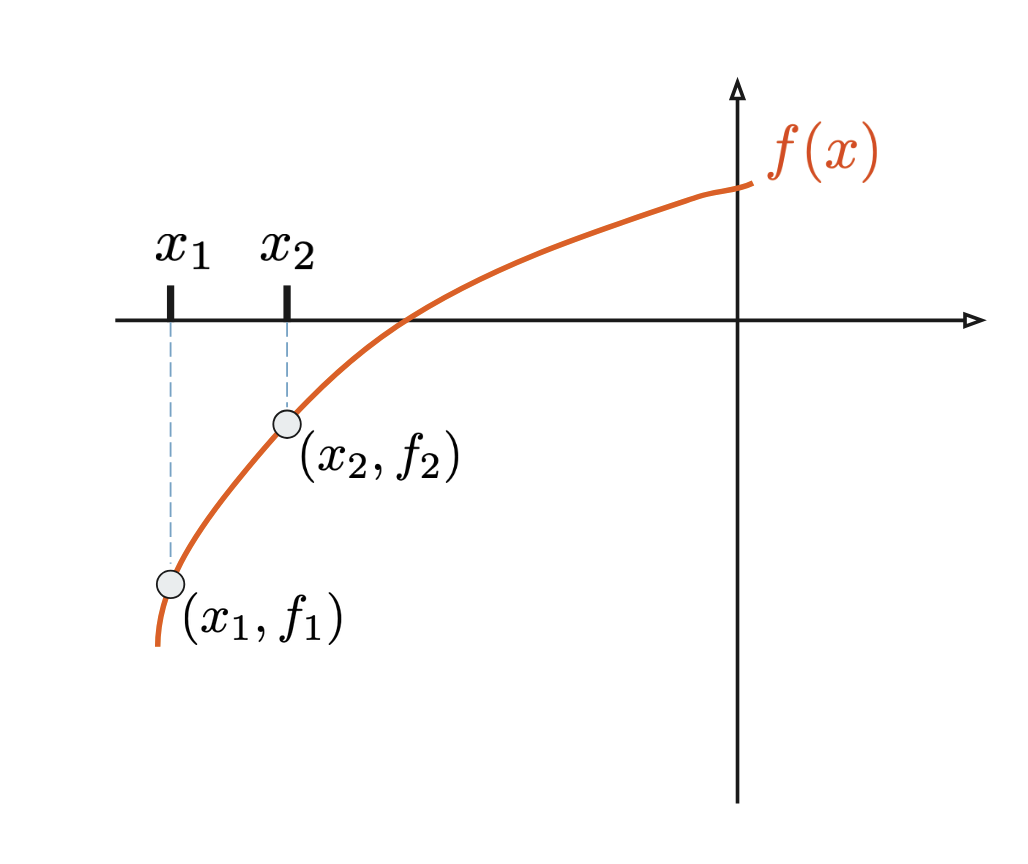
\includegraphics[width=3.64583in,height=3.125in]{sec2.png}
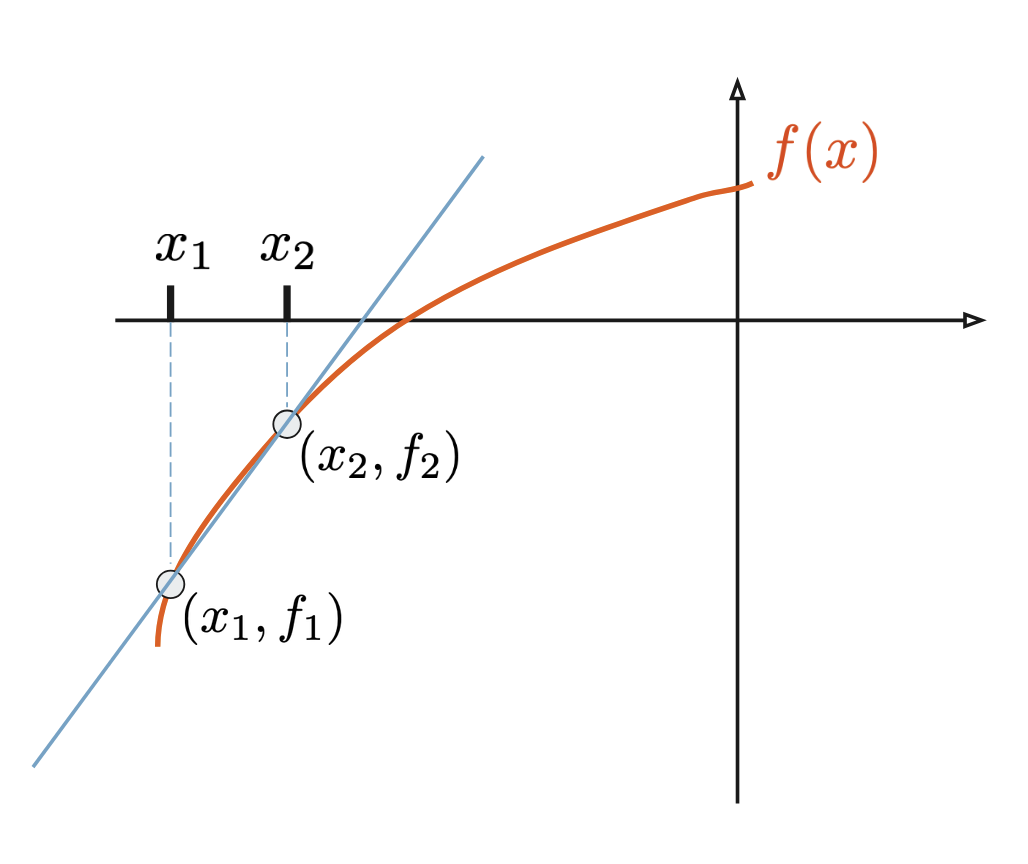
\includegraphics[width=3.64583in,height=3.125in]{sec3.png}
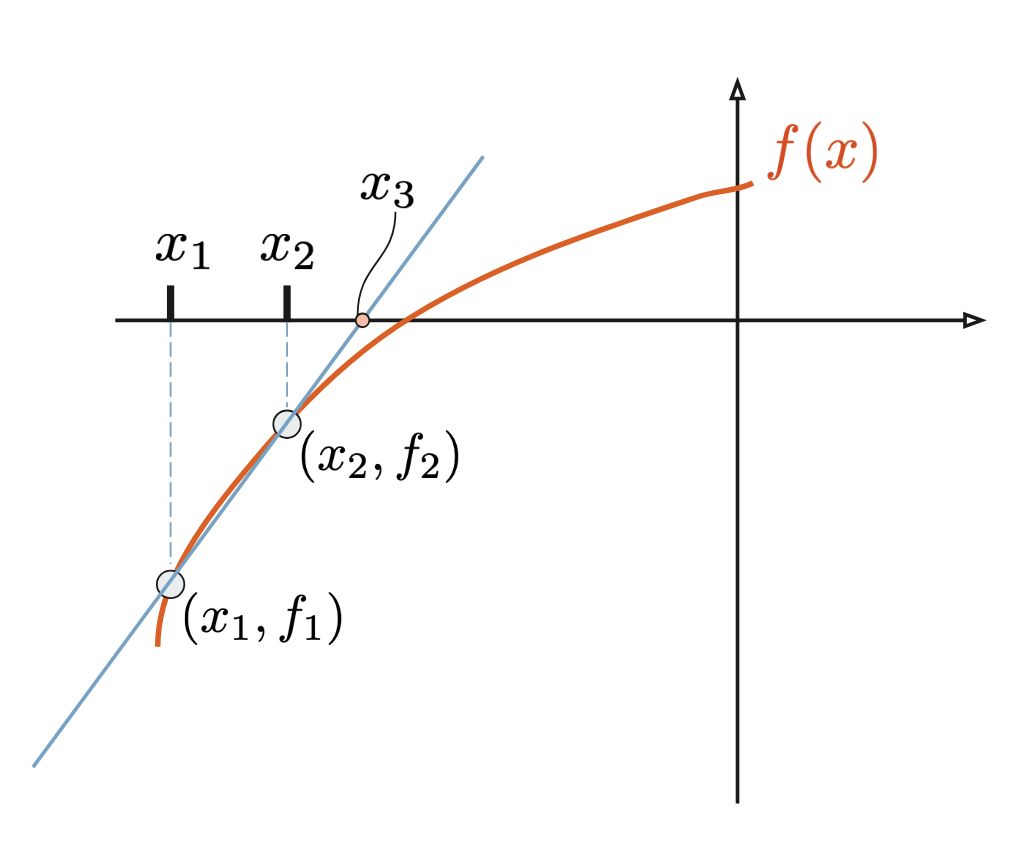
\includegraphics[width=3.64583in,height=3.125in]{sec4.png}
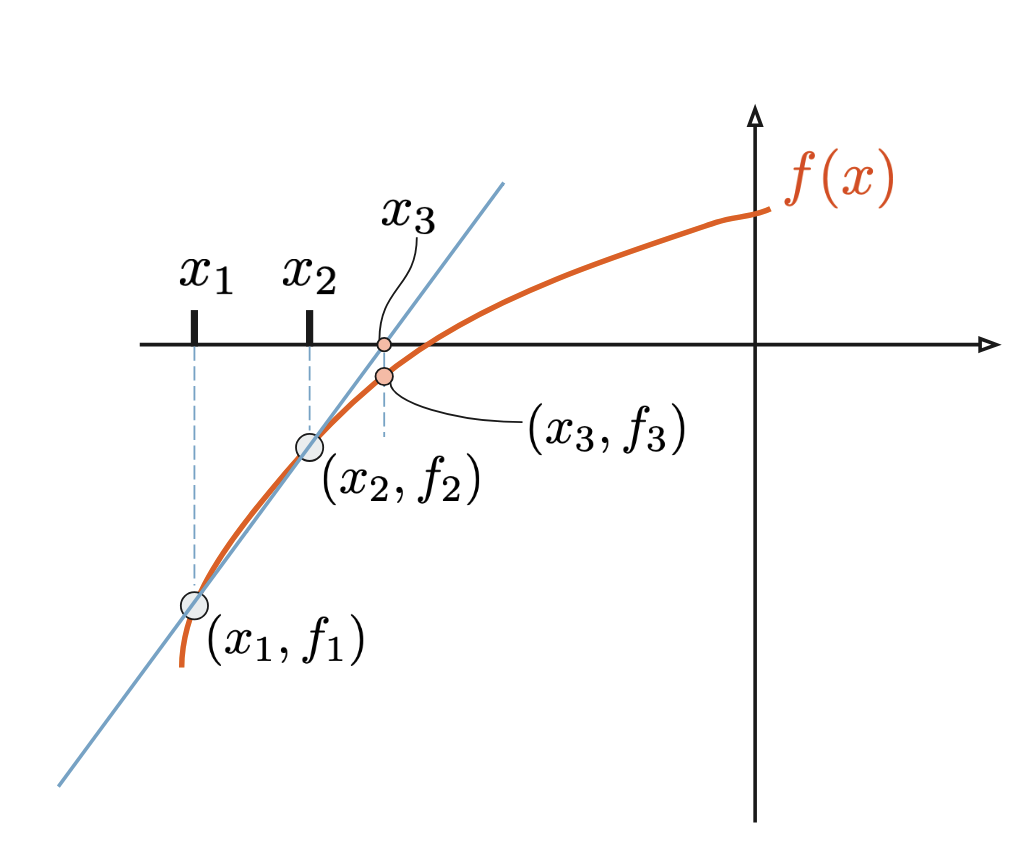
\includegraphics[width=3.64583in,height=3.125in]{sec5.png}

\subsubsection{Writing a program for the Secant
method}\label{writing-a-program-for-the-secant-method}

\begin{Shaded}
\begin{Highlighting}[]
\ImportTok{from}\NormalTok{ numpy }\ImportTok{import}\NormalTok{ linspace}
\KeywordTok{def}\NormalTok{ f(x):}
    \ControlFlowTok{return} \OperatorTok{{-}}\NormalTok{(x}\OperatorTok{+}\FloatTok{1.5}\NormalTok{)}\OperatorTok{*}\NormalTok{(x}\OperatorTok{+}\FloatTok{2.5}\NormalTok{)}

\NormalTok{x1 }\OperatorTok{=} \OperatorTok{{-}}\DecValTok{2}
\NormalTok{x2 }\OperatorTok{=} \OperatorTok{{-}}\DecValTok{1}

\NormalTok{fx1 }\OperatorTok{=}\NormalTok{ f(x1)}
\NormalTok{fx2 }\OperatorTok{=}\NormalTok{ f(x2)}

\CommentTok{\# Find equation of straight line}
\CommentTok{\# thru (x1,fx1) and (x2,fx2)}

\NormalTok{m }\OperatorTok{=}\NormalTok{ (fx2}\OperatorTok{{-}}\NormalTok{fx1)}\OperatorTok{/}\NormalTok{(x2}\OperatorTok{{-}}\NormalTok{x1)}

\BuiltInTok{print}\NormalTok{(}\SpecialStringTok{f"Slope of the line btwn 2 points is }\SpecialCharTok{\{}\NormalTok{m}\SpecialCharTok{\}}\SpecialStringTok{"}\NormalTok{)}

\CommentTok{\# To find y{-}intercept, use one of the points}
\CommentTok{\# y = mx + c}
\CommentTok{\# fx1 = m*x1 + c}
\CommentTok{\# c = fx1 {-} m*x1}
\NormalTok{c }\OperatorTok{=}\NormalTok{ fx1 }\OperatorTok{{-}}\NormalTok{ m}\OperatorTok{*}\NormalTok{x1}

\CommentTok{\# equation of straight line is y = mx + c}

\CommentTok{\# Now find the point where this line intscts}
\CommentTok{\# the x{-}axis}

\CommentTok{\# y = mx + c}
\CommentTok{\# 0 = m*x\_intercept + c}
\CommentTok{\# x\_intercept = {-} c/m}
\NormalTok{x\_int }\OperatorTok{=} \OperatorTok{{-}}\NormalTok{c}\OperatorTok{/}\NormalTok{m}

\BuiltInTok{print}\NormalTok{(}\SpecialStringTok{f"The line intersects x{-}axis at }\SpecialCharTok{\{}\NormalTok{x\_int}\SpecialCharTok{\}}\SpecialStringTok{"}\NormalTok{)}
\end{Highlighting}
\end{Shaded}

\subsubsection{Newton's Method}\label{newtons-method}

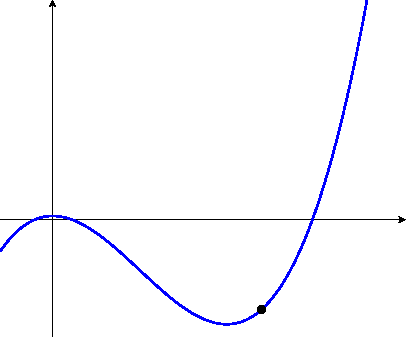
\includegraphics[width=6in,height=\textheight,keepaspectratio]{index_files/mediabag/tikz.f836b544.pdf}

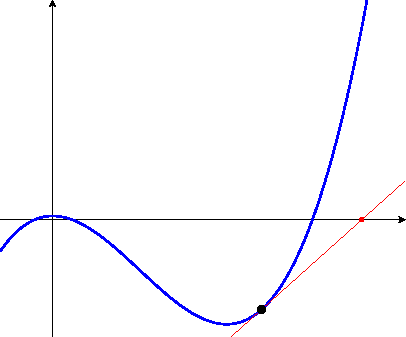
\includegraphics[width=6in,height=\textheight,keepaspectratio]{index_files/mediabag/tikz.007c58be.pdf}

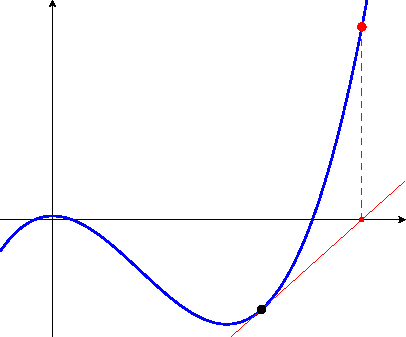
\includegraphics[width=6in,height=\textheight,keepaspectratio]{index_files/mediabag/tikz.3f6dd931.pdf}

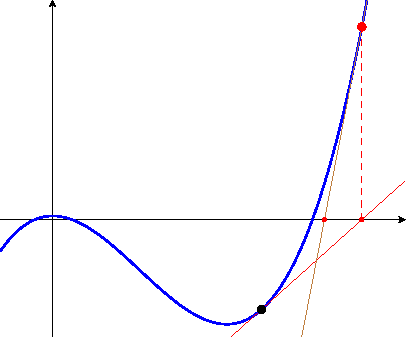
\includegraphics[width=6in,height=\textheight,keepaspectratio]{index_files/mediabag/tikz.fec98bd8.pdf}

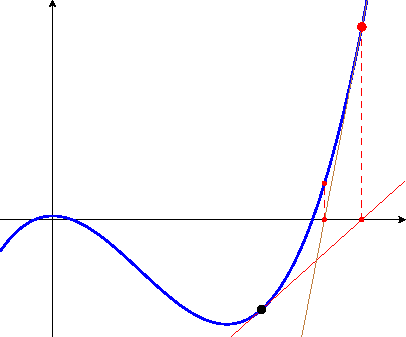
\includegraphics[width=6in,height=\textheight,keepaspectratio]{index_files/mediabag/tikz.98064aa7.pdf}

\subsubsection{Summary of Newton's
Method}\label{summary-of-newtons-method}

{Evaluate the function at your first guess.}

{Make a straight line tangent to \((x_1,f_1)\)}

{Find location where this line intersects x-axis. This is the 2nd guess,
call it \(x_2\).}

{Repeat.}

\includegraphics[width=3.64583in,height=3.125in]{newt1.png}
\includegraphics[width=3.64583in,height=3.125in]{newt2.png}
\includegraphics[width=3.64583in,height=3.125in]{newt3.png}
\includegraphics[width=3.64583in,height=3.125in]{newt4.png}

\subsubsection{Comparing Newton's method with Secant
method}\label{comparing-newtons-method-with-secant-method}

\begin{itemize}
\tightlist
\item
  Newton's method for finding roots of \(f(x)\) requires that you know
  \(f'(x)\) already.
\item
  Secant method requires starting with two points instead of one.
\item
  If two points very close to each other are chosen for the Secant
  method, the two methods are nearly identical
\end{itemize}

\subsubsection{Equations for Newton's
method}\label{equations-for-newtons-method}

{Derive an equation for \(x_{n+1}\) given \(x_n\)}

{Equation of the tangent line is \(y = mx+c\),}

{where \(m = f'(x_n)\). So we get \[y = f'(x_n) x + c\]}

{and \(c\) can be found by substituting a known point into the
equation:}

{\(\underbrace{f(x_n)}_{\text{y coordinate}} = f'(x_n) \underbrace{x_n}_{\text{x coordinate}} + c \implies c = f(x_n) - f'(x_n) x_n\).}

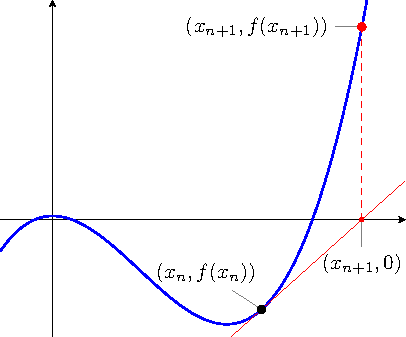
\includegraphics[width=6in,height=\textheight,keepaspectratio]{index_files/mediabag/tikz.4c0297aa.pdf}

{Thus, the equation of the straight line is
\(\displaystyle{\color{red}{y}} = \overbrace{f'(x_n)}^{m} {\color{red}{x}} + \overbrace{f(x_n) - f'(x_n) x_n}^{c}\)}

{The intersection of this line with the \(x\) axis occurs when \(y=0\),
i.e.:}

{\(0 =f'(x_n) {\color{red}{x}} + f(x_n) - f'(x_n) x_n\)}

{Recognizing that the unknown \({\color{red}{x}}\) is \(x_{n+1}\), we
get
\[f'(x_n) x_n - f(x_n)= f'(x_n) {\color{red}{x}} \implies \frac{f'(x_n) x_n - f(x_n)}{f'(x_n)} = {\color{red}{x}}\]}

{\[\implies \boxed{x_{n+1} = x_n - \frac{f(x_n)}{f'(x_n)}}\]}

\subsubsection{Writing a program for Newton's
method}\label{writing-a-program-for-newtons-method}

\subsubsection{Pitfalls of Root Finding}\label{pitfalls-of-root-finding}

If a root-finding program does not find a solution, it could be because:

\begin{enumerate}
\def\labelenumi{\arabic{enumi}.}
\tightlist
\item
  the equation \(f(x)=0\) has no solution
\item
  a solution exists but the program wasn't able to find it
\item
  a solution is found but it's not the desired solution
\item
  too many iterations are needed to arrive at the solution
\end{enumerate}

{A well-executed numerical method can solve problems 2-4 but cannot
solve problem 1.}

\subsubsection{Example --- Finding the wrong
root}\label{example-finding-the-wrong-root}

Suppose an equation is known to have multiple solutions, but only one of
them is physically meaningful. A root-finding program will not
necessarily find the solution we care about.

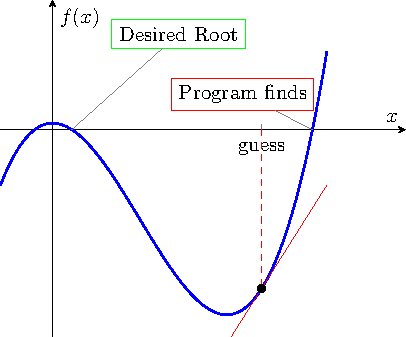
\includegraphics[width=6in,height=\textheight,keepaspectratio]{index_files/mediabag/tikz.09ebf14f.pdf}

\subsubsection{Example --- Stuck in a flat
place}\label{example-stuck-in-a-flat-place}

In the neighborhood of zero-slope points, these methods run into
problems.

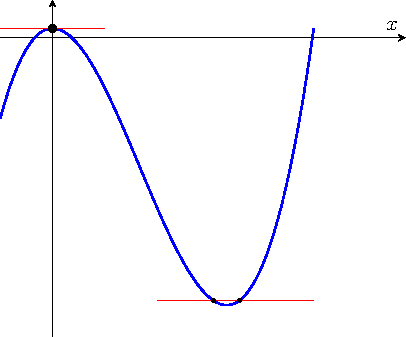
\includegraphics[width=6in,height=\textheight,keepaspectratio]{index_files/mediabag/tikz.76d1b64e.pdf}




\end{document}
